\subsection{Результаты в среде LunarLander}

Эксперименты в среде LunarLander стали ключевым этапом практического исследования, позволившим оценить работу когнитивных агентов в условиях сложного пространства состояний и необходимости тонкого микроконтроля. В отличие от базовой задачи CartPole, здесь перед агентами стояла цель не просто удержания баланса, а поиска оптимальной траектории посадки в условиях меняющейся гравитации и внешних возмущений.


\subsubsection{Сравнительный анализ архитектурной сложности и обучения}

В ходе исследования был зафиксирован значительный контраст в подходах к формированию управляющей политики:

\begin{figure}[h!] % [h!] - попытка разместить картинку "здесь" (here)
  \centering
  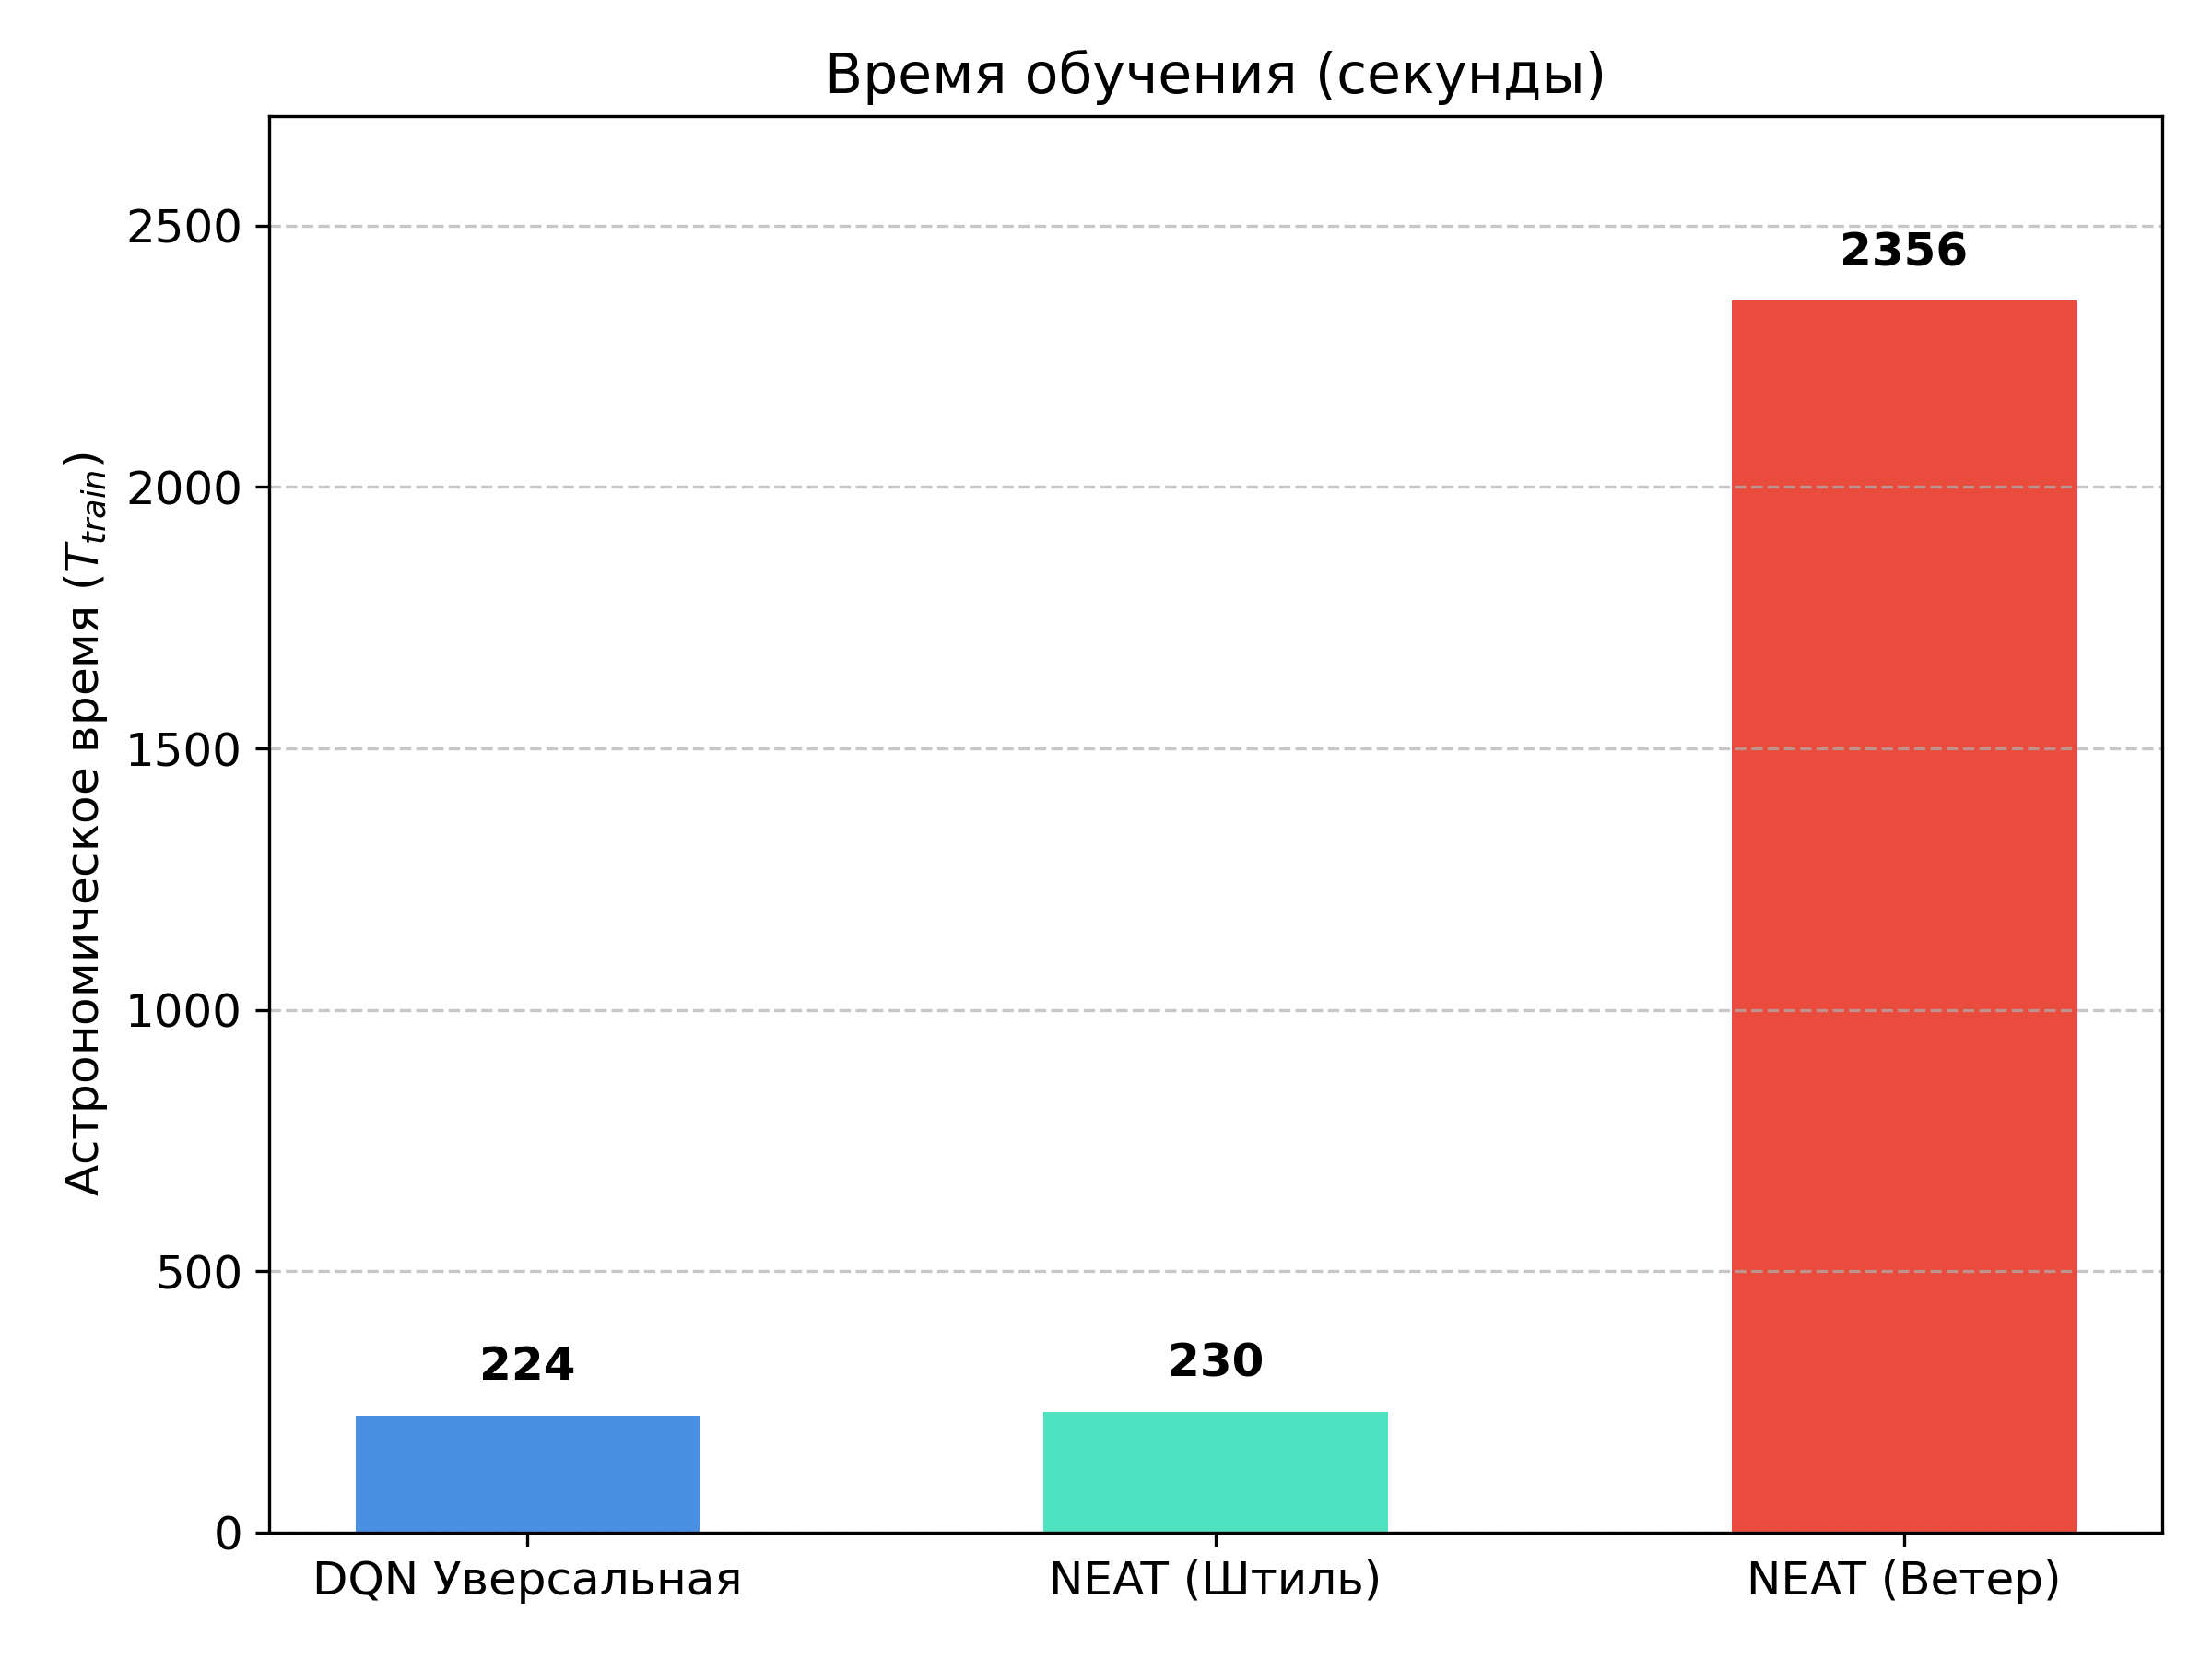
\includegraphics[width=0.6\textwidth]{./images/lunarlander_speed.png}
  
  \caption{Скорость схождения двух алгоритмов.}
  \label{fig:lunarlander_speed}
\end{figure}


Практика опять подтвердила гипотезу контрасте между тем, как алгоритмы формируют управляющую политику. Если смотреть на скорость схождения на рисунке \ref{fig:lunarlander_speed}, то алгоритм DQN оказался явным лидером, потому что пробил целевой порог приспособленности (>200) всего за 170 000 шагов взаимодействия со средой, что заняло около 224 секунд реального времени. Нейроэволюционному подходу потребовалось куда больше итераций для поиска рабочей топологии.  Однако эта задержка на этапе обучения полностью окупается в момент инференса. Итоговая информационная емкость моделей отличается на порядки, что можно увидеть на рисунке \ref{fig:lunarlander_complexity}. Для достижения стабильных результатов DQN-агенту понадобилась тяжеловесная глубокая сеть размерностью [512, 512], содержащая 69 124 обучаемых параметра. NEAT же, напротив, вырастил очень компактный граф всего из 150–200 связей и узлов.

\subsubsection{Феномен «нейролоботомии» и проблема локальных оптимумов}

Во время симуляций мы столкнулись с весьма специфическим побочным эффектом, который условно классифицировали как «нейролоботомию». Из-за того, что среда накладывает жесточайший штраф за крушение модуля в -100 очков, самый безопасный выход для развития адаптации агента к среде, но не менее деструктивный выход стал в том, чтобы вообще ничего не делать. Агент буквально обрывал связи в собственной сети и отключал двигатели, лишь бы не совершить фатальную ошибку при активном маневрировании. Статистически алгоритму было выгоднее просто падать вниз, чем пытаться управлять модулем и разбиваться. Чтобы вытащить сеть из этого локального оптимума, нам пришлось перенастраивать функции приспособленности и добавлять элементы рандомизации в стартовые условия.

\subsubsection{Устойчивость в условиях неопределенности и внешних шумов}

\begin{figure}[h!] % [h!] - попытка разместить картинку "здесь" (here)
  \centering
  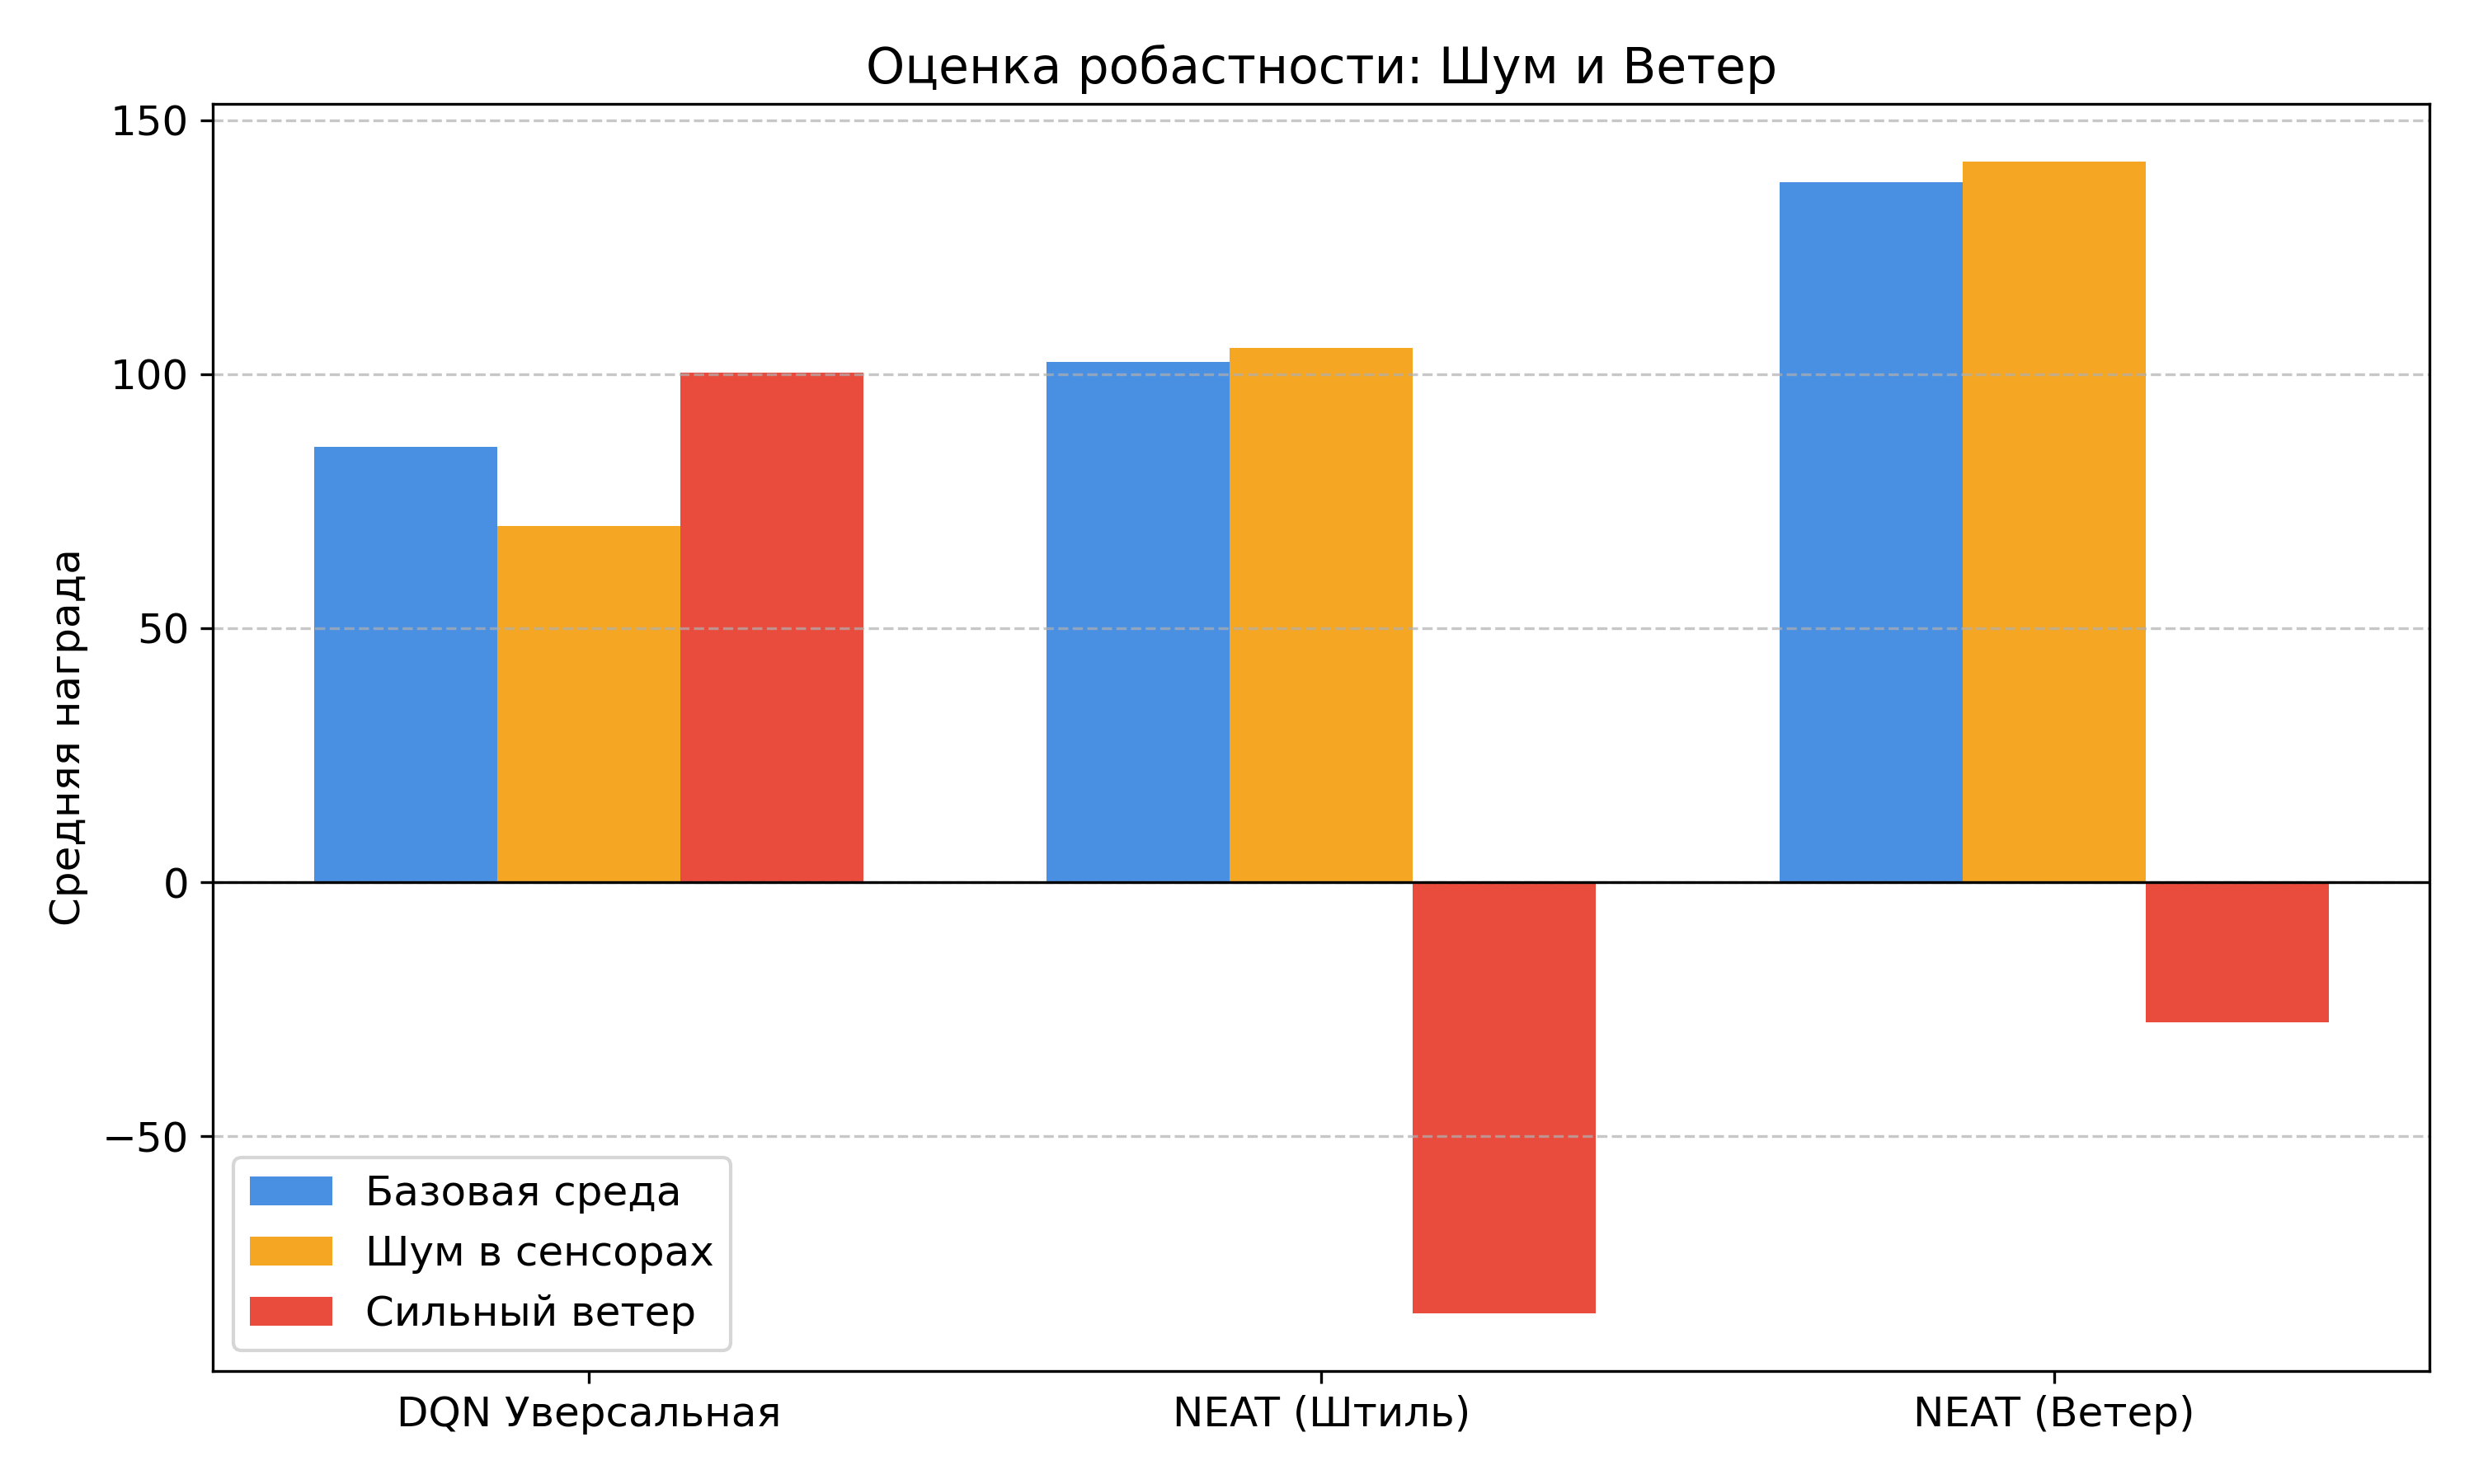
\includegraphics[width=0.6\textwidth]{./images/lunarlander_robustness.png}
  
  \caption{Устойчивость двух алгоритмов.}
  \label{fig:lunarlander_robustness}
\end{figure}

Отдельной задачей стало стресс-тестирование агентов на устойчивость к внешним возмущениям вроде турбулентности или бокового ветра. Для DQN пришлось написать специальную обертку UniversalWindWrapper, которая в половине эпизодов генерировала порывы ветра мощностью до 20.0. Это вынуждало полносвязную сеть искать паттерны компенсации смещения. С алгоритмом NEAT мы поступили иначе: заставили каждый геном сдавать серию из 5 испытаний (EPISODES\_PER\_GENOME = 5), где штиль чередовался с непогодой. Итоговая оценка суммировалась, а фактор случайного везения сводился к нулю. 

Сводные результаты этих тестов на рисунке \ref{fig:lunarlander_robustness} показывают, что универсальная DQN-модель отлично справляется в идеальных условиях, набирая 85.75, но слаба перед шумами в сенсорах, проседая по эффективности до 70.13. В то же время NEAT показал хорошую стабильность к высокочастотным помехам из-за низкой сложности архитектуры нейросети.

\subsubsection{Специфика программной реализации}

Чтобы гарантировать научную достоверность и воспроизводимость всех экспериментов, мы строго контролировали генерацию случайных чисел. Это ставило всю популяцию из 150-300 агентов в абсолютно идентичные стартовые условия, делая эволюционный отбор полностью равным. А учитывая тяжелую физику LunarLander и необходимость пятикратной проверки каждой особи, мы распараллелили вычисления по ядрам процессора через модуль multiprocessing.

\subsubsection{Практические выводы}

Классический подход DQN — это отличный выбор для быстрого обучения в детерминированной среде с высокой размерностью данных. Но если речь заходит о создании устойчивых систем управления, которым предстоит работать в условиях неопределенности и жесткого дефицита вычислительных ресурсов, нейроэволюция оказывается гораздо более предпочтительным инструментом.